%!TEX root = ../notes.tex
\section{February 7, 2023}
\subsection{Natural Numbers, \emph{continued}}
\begin{theorem}
    Let $S$ be an infinite subset of $\NN$. Then $S$ is countably infinite.
\end{theorem}
\begin{proof}
    The objective is to construct a bijection between $S$ and $\NN$. We will do this inductively.

    Let $f(1)$ be the smallest element\footnote{Within resonable context, we assume that $\NN$ is well-ordered. That is, every subset has a least element.} of $S$ for $f : \NN\to S$.

    Assuming we have defined $f(1), f(2), \dots, f(n)$, we define $f(n+1)$ to be the smallest element of $S \setminus \{f(1), f(2), \dots, f(n)\}$.

    By construction, $f$ is bijective.
\end{proof}

Recall \cref{defn:countability}:
\begin{definition*}[Countability]
    We say that $A$ is \ul{countable} if it is finite or countably infinite.
\end{definition*}

\begin{theorem}
    Let $\mathcal{C}$ be a countable collection\framedfootnote{A `collection' usually refers to a collection of sets.} of countable sets.

    Then the union $\displaystyle \bigcup_{A\in \mathcal{C}}A$ is countable.
\end{theorem}

We can do something like this:
\begin{center}
    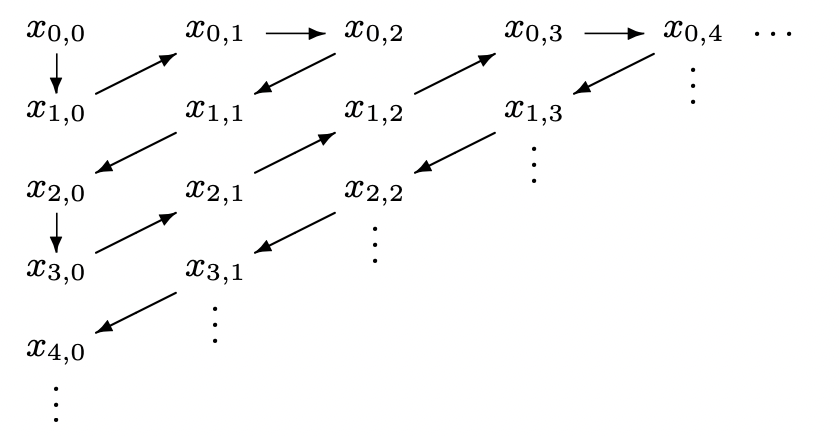
\includegraphics[width=0.5\textwidth]{images/countable_collection_of_sets.png}
\end{center}

\begin{proof}
    Again, we try to construct a bijection $f$ from $\NN$. We list all the elements of $\bigcup_{A\in\cC}A$ in a sequence. This will give $f(1), f(2), \dots$ and so on.

    Since each $A$ is countable, we may list its elements. The collection $\cC$ is also countable. We can arrange every row to be an element of $\cC$.


    \[\begin{array}{c|cccc}
            A_1    & a_1    & a_2    & a_3    & \cdots \\
            A_2    & b_1    & b_2    & b_3    & \cdots \\
            A_3    & c_1    & c_2    & \cdots          \\
            A_4    & d_1    & \cdots                   \\
            \vdots & \vdots & \ddots
        \end{array}\]

    We then count the elements using diagonals (or a zig-zag), and remove duplicates\footnote{This is a bit wishy-washy, but we're only removing elements here so we remain in the `countable' territory.}.
\end{proof}

\subsection{Before We Get to the Real Numbers}
Let's begin by proving the following theorem.
\begin{theorem}
    $\sqrt{2}$ is not rational.
\end{theorem}
\begin{proof}
    Assume not, that we can write $\sqrt{2} = \frac{m}{n}$, for $m, n\in\ZZ$, $N\neq 0$ and $m, n$ coprime.

    Then, $2n^2 = m^2$. So, $m$ is even. Writing $m = 2m'$, $2n^2 = 4m'^2$, which in particular implies $n$ is even, which is a contradiction.

    It had better be, then, that $\sqrt{2}$ is irrational.
\end{proof}

We now show more, namely that we can get arbitrarily close to irrational numbers by rational numbers\footnote{This is to say, $\QQ$ is \emph{dense} in $\RR$.}.
\begin{theorem}
    If $q\in\QQ$ satisfies $0 < q^2 < 2$, then we can find $\bar{q}\in\QQ$ such that $q^2 < \bar{q}^2 < 2$. Similarly if $r\in\QQ$ satisfies $2 < r^2$, then we can find $\bar{r}\in\QQ$ such that $2 < \bar{r}^2 < r^2$.
\end{theorem}
\begin{proof}
    We'll just prove the first part; the second part is similar.

    Suppose $q > 0$, define
    \[\bar{q} = q + \frac{2 - q^2}{2 + q}.\]
    then $\bar{q} > q$ and
    \begin{align*}
        \bar{q}^2 - 2 & = q^2 + \left( \frac{2-q^2}{q+2} \right)^2 + \frac{2q(2-q^2)}{2+q} - 2                                       \\
                      & = \frac{(q^2 - 2)(q+2)^2 + (2-q^2)^2 + (2-q^2)2q(2+q)}{(q+2)^2}                                              \\
                      & = \frac{q^2 - 2}{(q+2)^2}\left[ \cancel{q^2} + 4 + \cancel{4q} + \cancel{q^2} - 2 - \cancel{2q(2+q)} \right] \\
                      & = \frac{2(q^2 - 2)}{(q+2)^2}
    \end{align*}
    which is surely negative.
\end{proof}
\begin{corollary}
    The set
    \[\left\{ q\in\QQ\mid q^2 < 2 \right\}\]
    \textbf{does not} have a largest element.
\end{corollary}

\begin{definition}[Upper Bound]
    If $A$ is a set with a partial ordering $\leq$, we say that $a\in A$ is an \ul{upper bound} for a subset $B\subset A$ if $b\leq a$ $\forall b\in B$.

    We say that $a$ is a \ul{least upper bound} for $B$ if whenever $a'$ is an upper bound for $B$, then $a\leq a'$.
\end{definition}

\begin{lemma}
    If $a$ is a least upper bound for $B$, then $a$ is unique.
\end{lemma}
\begin{proof}
    Assume $a, a'$ are both least upper bounds for $B$. By definition, both $a, a'$ are upper bounds. \textsc{wlog}, if $a$ is a least upper bound and $a'$ an upper bound, $a\leq a'$. Similarly, $a'\leq a$. Hence, $a = a'$.
\end{proof}
Now that we have proved uniqueness, we can give $a$ a name:
\begin{definition}[Supremum \& Infimum]
    We define $\sup B := a$ when $a$ is the least upper bound of $B$.

    Similarly, $\inf B := a$ when $a$ is the greatest lower bound of $B$.
\end{definition}
\begin{definition}[Least-Upper-Bound Property]
    Let $A$ be a totally ordered set with order $\leq$. We say that $A$ has the least upper bound property if each nonempty subset of $B\subset A$ with an upper bound in $A$ has a least upper bound in $A$.
\end{definition}

% \intentionalpagebreak
\subsection{The Real Numbers}

\begin{definition}
    A \ul{field} $F$ is a set with two operations: $+, \cdot$.

    The $+$ operation satisfies:
    \begin{description}
        \item[Closure.] $x, y\in F\Rightarrow x + y\in F$.
        \item[Commutativity.] $x + y = y + x$, $\forall x, y\in F$.
        \item[Associatifity.] $(x + y) + z = x + (y + z)$, $\forall x, y, z\in F$.
        \item[Identity.] $\exists 0$ such that $0 + x = x$ $\forall x\in F$.
        \item[Inverses.] $\forall x\in F$, $\exists -x\in F$ such that $x + (-x) = 0$.
    \end{description}

    And a $\cdot$ operation that satisfies:
    \begin{description}
        \item[Closure.] $x, y\in F\Rightarrow x \cdot y\in F$.
        \item[Commutativity.] $x \cdot y = y \cdot x$, $\forall x, y\in F$.
        \item[Associatifity.] $(x \cdot y) \cdot z = x \cdot (y \cdot z)$, $\forall x, y, z\in F$.
        \item[Identity.] $\exists 1 \neq 0$ such that $1\cdot x = x$, $\forall x\in F$.
        \item[Inverse.] $\forall x\neq 0$, $\exists x^{-1}\in F$ such that $x\cdot x^{-1} = 1$
    \end{description}

    Together, we also have
    \begin{description}
        \item[Distribution.] $\forall x, y, z\in F$, $x\cdot (y + z) = x\cdot y + x\cdot z$.
    \end{description}

    In other words, a field $F$ is a commutative ring with multiplicative inverse.
\end{definition}
\begin{definition}
    An \ul{ordered field} is a field $F$ which is an ordered set such that
    \begin{enumerate}
        \item $x + y < x + z$ if $x, y, z\in F$ and $y < z$.
        \item $x\cdot y > 0$ if $x, y\in F$ and $x > 0$, $y > 0$.
    \end{enumerate}
\end{definition}
\begin{example}
    $\QQ, \RR$ are ordered fields. $\NN, \ZZ$ are not fields.
\end{example}

\begin{theorem}[Archimedian Property]
    \label{thm:archimedian-property}
    Given $x, y\in \RR$, $x > 0$. Then $\exists n\in \ZZ$ such that $nx > y$.
\end{theorem}
\begin{proof}
    We argue by contradiction. Assume such $n$ doesn't exists.

    Then take set
    \[A = \left\{ nc \mid n\in\NN \right\}\]
    which is bounded by $y$.

    Therefore, if it has supremum\footnote{$\RR$ has the least upper bound property.} $s$, $s-x < s$, so $s-x$ is not an upper bound of $A$ (otherwise $s$ is not a supremum). Then, $\exists a\in A$ (otherwise $s-x$ would have been an upper bound) such that $a \geq s - x$, which means $\exists m\in \NN$ such that $mx > s-x$. This implies that $s < (m+1)x$ but $m+1\in A$, which is a contradiction.
\end{proof}

\begin{corollary}
    Let $x, y\in\RR$ with $x < y$. Then $\exists q\in \QQ$ such that $x < q < y$. This is to say, ``in between any two real numbers lies rational numbers.''
\end{corollary}
\begin{proof}
    By \cref{thm:archimedian-property} applied to $y-x$ and $1$. Then $\exists n\in\ZZ$ such that
    \[n(y-x) > 1\]
    and we can also find $m_1, m_2\in\NN$ such that
    \[m_1 > nx, m_2 > -nx\]
    by the Archimedian property again.
    which implies
    \[-m_2 < nx < m_1\]
    Then, $\exists m\in \NN$ such that $m-1 \leq nx < m$\footnote{By contradiction, if there is no such $m$ we incur the previous statement}. Which implies that
    \[nx < m \leq 1 + nx < ny\]
    which then gives
    \[x < \frac{m}{n} < y\]
    which is as desired. $\frac{m}{n}$ is precisely a rational between real $x$ and $y$.
\end{proof}

\begin{theorem}
    For every $x\in\RR$ with $x > 0$, $n > 0\in \NN$, $\exists! y > 0$ such that $y^n = x$.
\end{theorem}
\begin{proof}
    We prove uniqueness. Suppose by contradiction that \textsc{wlog} $y_1 < y_2$ such that $y_1 ^ n = x$ and $y_2^n = x$. Contradiction by $y_1^n < y_2^n$.

    We now start the proof for existence. Let
    \[E = \{t\mid t^n < x\}\]
    If $t = \frac{x}{x+1}$, then $t < x$ and $0 < t < 1$. So $t^n < t < x$ so $E$ is not empty.

    If $t > 1 + x$, $t^n \geq t > x$. We've found an upper bound of $E$. Then, $\exists y = \sup E$.

    We'll leave it here that $E$ has a supremum, and continue next time.
\end{proof}